\chapter{Implemented Solution}

\section{Amazon Web Services}

\subsection{Architecture}
\begin{figure}[h]
    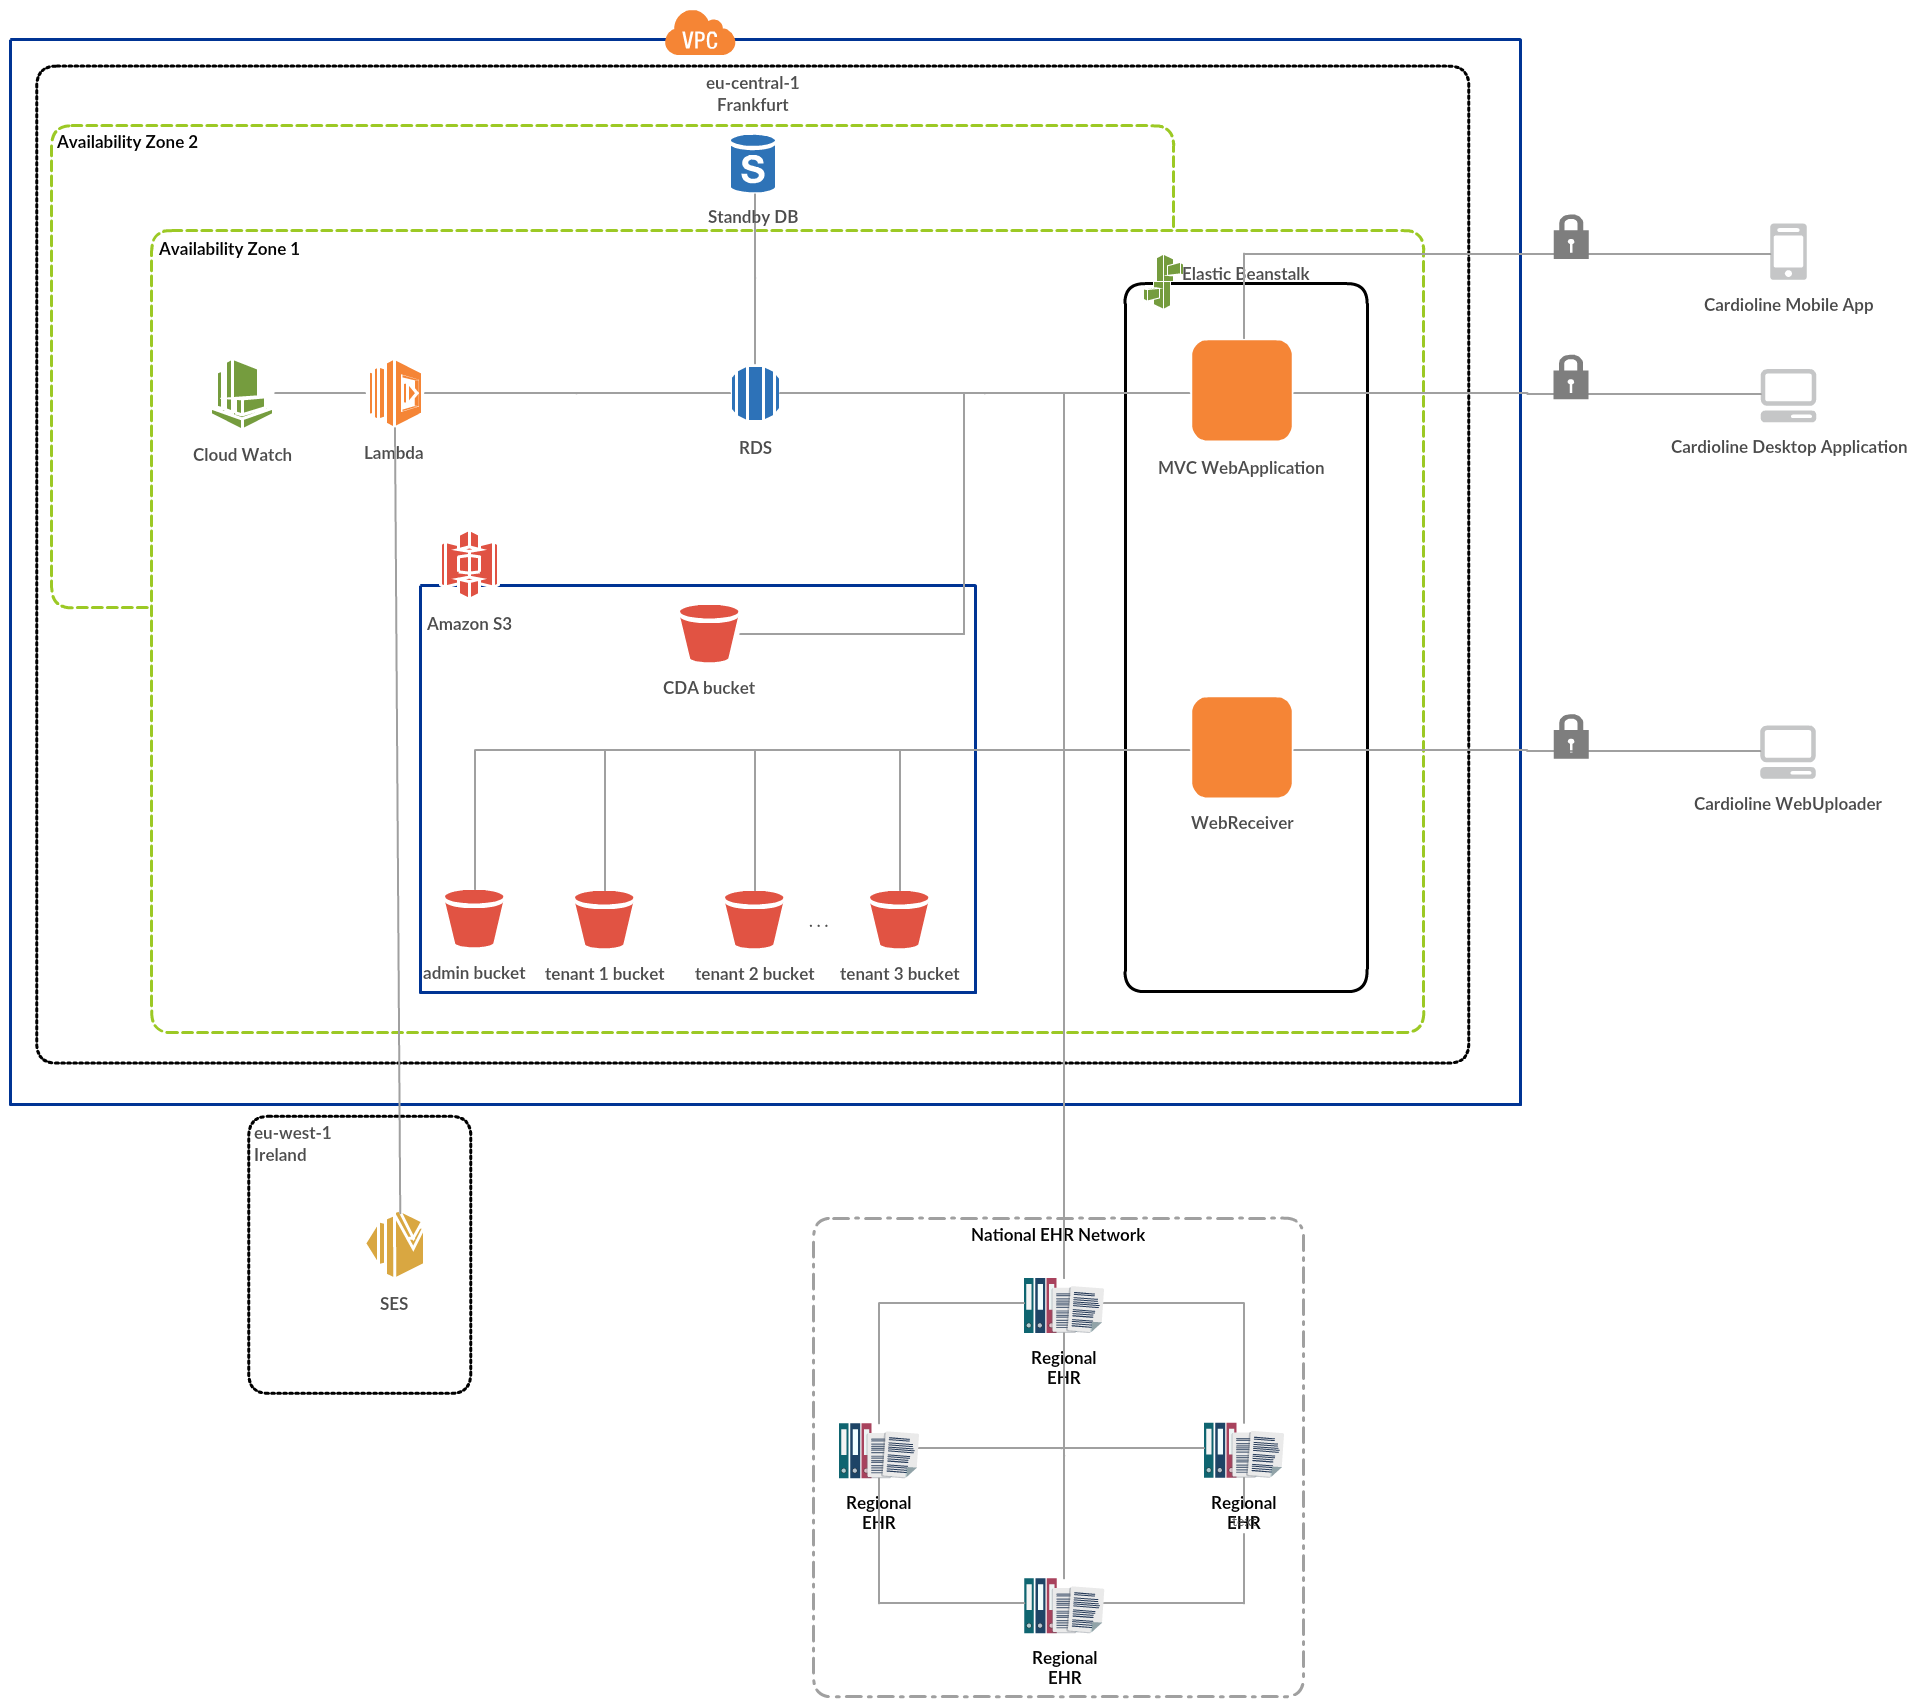
\includegraphics[width=\textwidth]{img/architecture}
    \caption{Architecture Scheme}
    \label{fig:architecture}
\end{figure}
Since Amazon Elastic Beanstalk (EB) has been used as the core component of the system, it has been possible to use an Infrastructure as a Service (IaaS \ref{paragraph:Iaas}) grade of customization, with an easier configuration and building phase as if the system was Platform as a Service (PaaS \ref{paragraph:Paas}) instead.\\
As shown in picture \ref{fig:architecture}, everything but the Amazon Simple Email Service (SES \cite{AmazonSes}) service is hosted in the eu-central-1 region in Frankfurt to reduce latency, minimize costs and keep healthcare data in an European law venue, as in production would be.
The region is divided into availability zones connected each other with low-latency links, to handle potential instance failures by replacing them with the standby ones located in a different availability zone.\\
EB handles the WebServer instances: one for the EcgWebApp, more details in section \ref{paragraph:ecgwebapp} and the other one for Ecg WebReceiver,section \ref{paragraph:ecgwebreceiver}. The interaction is then allowed to authenticated users bounded to their capabilities and role.\\
The persistency is achieved by a Relational Database Service (RDS) running Amazon Aurora DB, a compatible MySql Database organized with a master write replica and several read replicas.
Furthermore, RDS provides a standby and synchronous Database, hosted in another availability zone, that is ready to become the new master in case of failure of the current master.\\
All the assets and static files are read and written from/to AWS S3 relative bucket.\\
The notification system is triggered by DB events and carried on by AWS Lambda functions using Amazon Simple Email Service (SES) as delivery service to final users. This service is not available in the Frankfurt region, hence the Ireland region was chosen.

\section{Ecg Workflow}
\label{section:ecgworkflow}
Resting Electrocardiogram (\ref{paragraph:Resting}) are uploaded from different device types such as mobile phones, desktop computers and Cardioline specific machines to EcgWebApp through a specific REST interface (details about REpresentational State Transter\ref{paragraph:REST}). The exam is stored in a \textit{pending} state and every associated physician notified for the anamnesis provisioning.
The user interface for a physician with anamnesis providing rights logged in is displayed in fig.\ref{fig:todo_anamnesi}.
Once the history of a \textit{pending} exam has been supplied (screenshot at fig.\ref{fig:aggiunta_anamnesi}) it passes to a \textit{ready} state. At this point every associated doctor with review role and permission, usually a cardiologist, is notified and allowed to write its own conclusion, as showed in figure \ref{fig:aggiunta_anamnesi}, and eventually ask for a second opinion from another expert. The exam state is finally set to \textit{confirmed} and the patient doctor notified.
\begin{figure}[h]
    \centering
    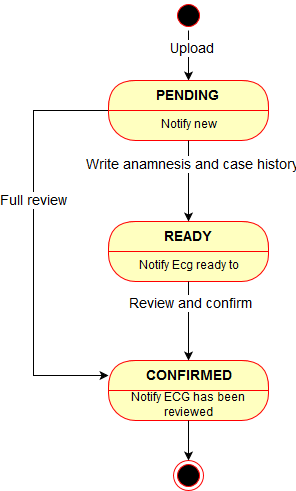
\includegraphics[width=6cm]{img/ECGstatechart}
    \caption{Electrocardiogram State Chart}
    \label{fig:ECGstatechart}
\end{figure}
\clearpage

\section{From ECG-SCP to EHR compliant document}
\label{section:from_ECG_SCP_to_EHR_compliant_document}
Subsequently to an expert review confirmation 
\subsection{CDA document}
\subsection{CDA from ECG-SCP builder module}
\paragraph{Resting}
\label{paragraph:Resting}
\paragraph{Cardiac stress test}
\label{paragraph:Cardiac stress test}
\paragraph{Holter}
\label{paragraph:Holter}

\section{Interoperability related architecture components}
The biggest contribution has been provided to the architecture components which interact with an external service. As it is possible to observe in figure \ref{fig:architecture} they are mainly two, EcgWebApp (\ref{paragraph:ecgwebapp}) for resting and cardiac stress test and Ecg WebReceiver (\ref{paragraph:ecgwebreceiver}) for Holter methodology.

\subsection{Web service and application}
These components instances are directly handled by Amazon Web Service Elastic Beanstalk (details at \ref{fig:architecture}): their load balancers and resources are dinamically allocated over the current request, load and configured parameters.\\
They both run on a 64-bit Windows Server 2012 R2 (with 32-bit compatibility) virtual machine executing IIS 8.5.
\paragraph{EcgWebApp}
\label{paragraph:ecgwebapp}
It's a 3-tier deployment architecture (\ref{fig:tiers_diagram}) based on Microsoft ASP .NET MVC framework. Its main components are:
\begin{itemize}
    \item \textit{WebBased UI and REST} - client interface
    \item \textit{WebServer} - handles http requests dispatching and routing to AppServer modules (IIS)
    \item \textit{Application Server} - ASP .NET Framework based business logic
    \item \textit{RDBMS (Relational Database Management System)} - Amazon Aurora and Amazon Simple Cloud Storage Service (S3)
\end{itemize}
\begin{figure}[h]
    \centering
    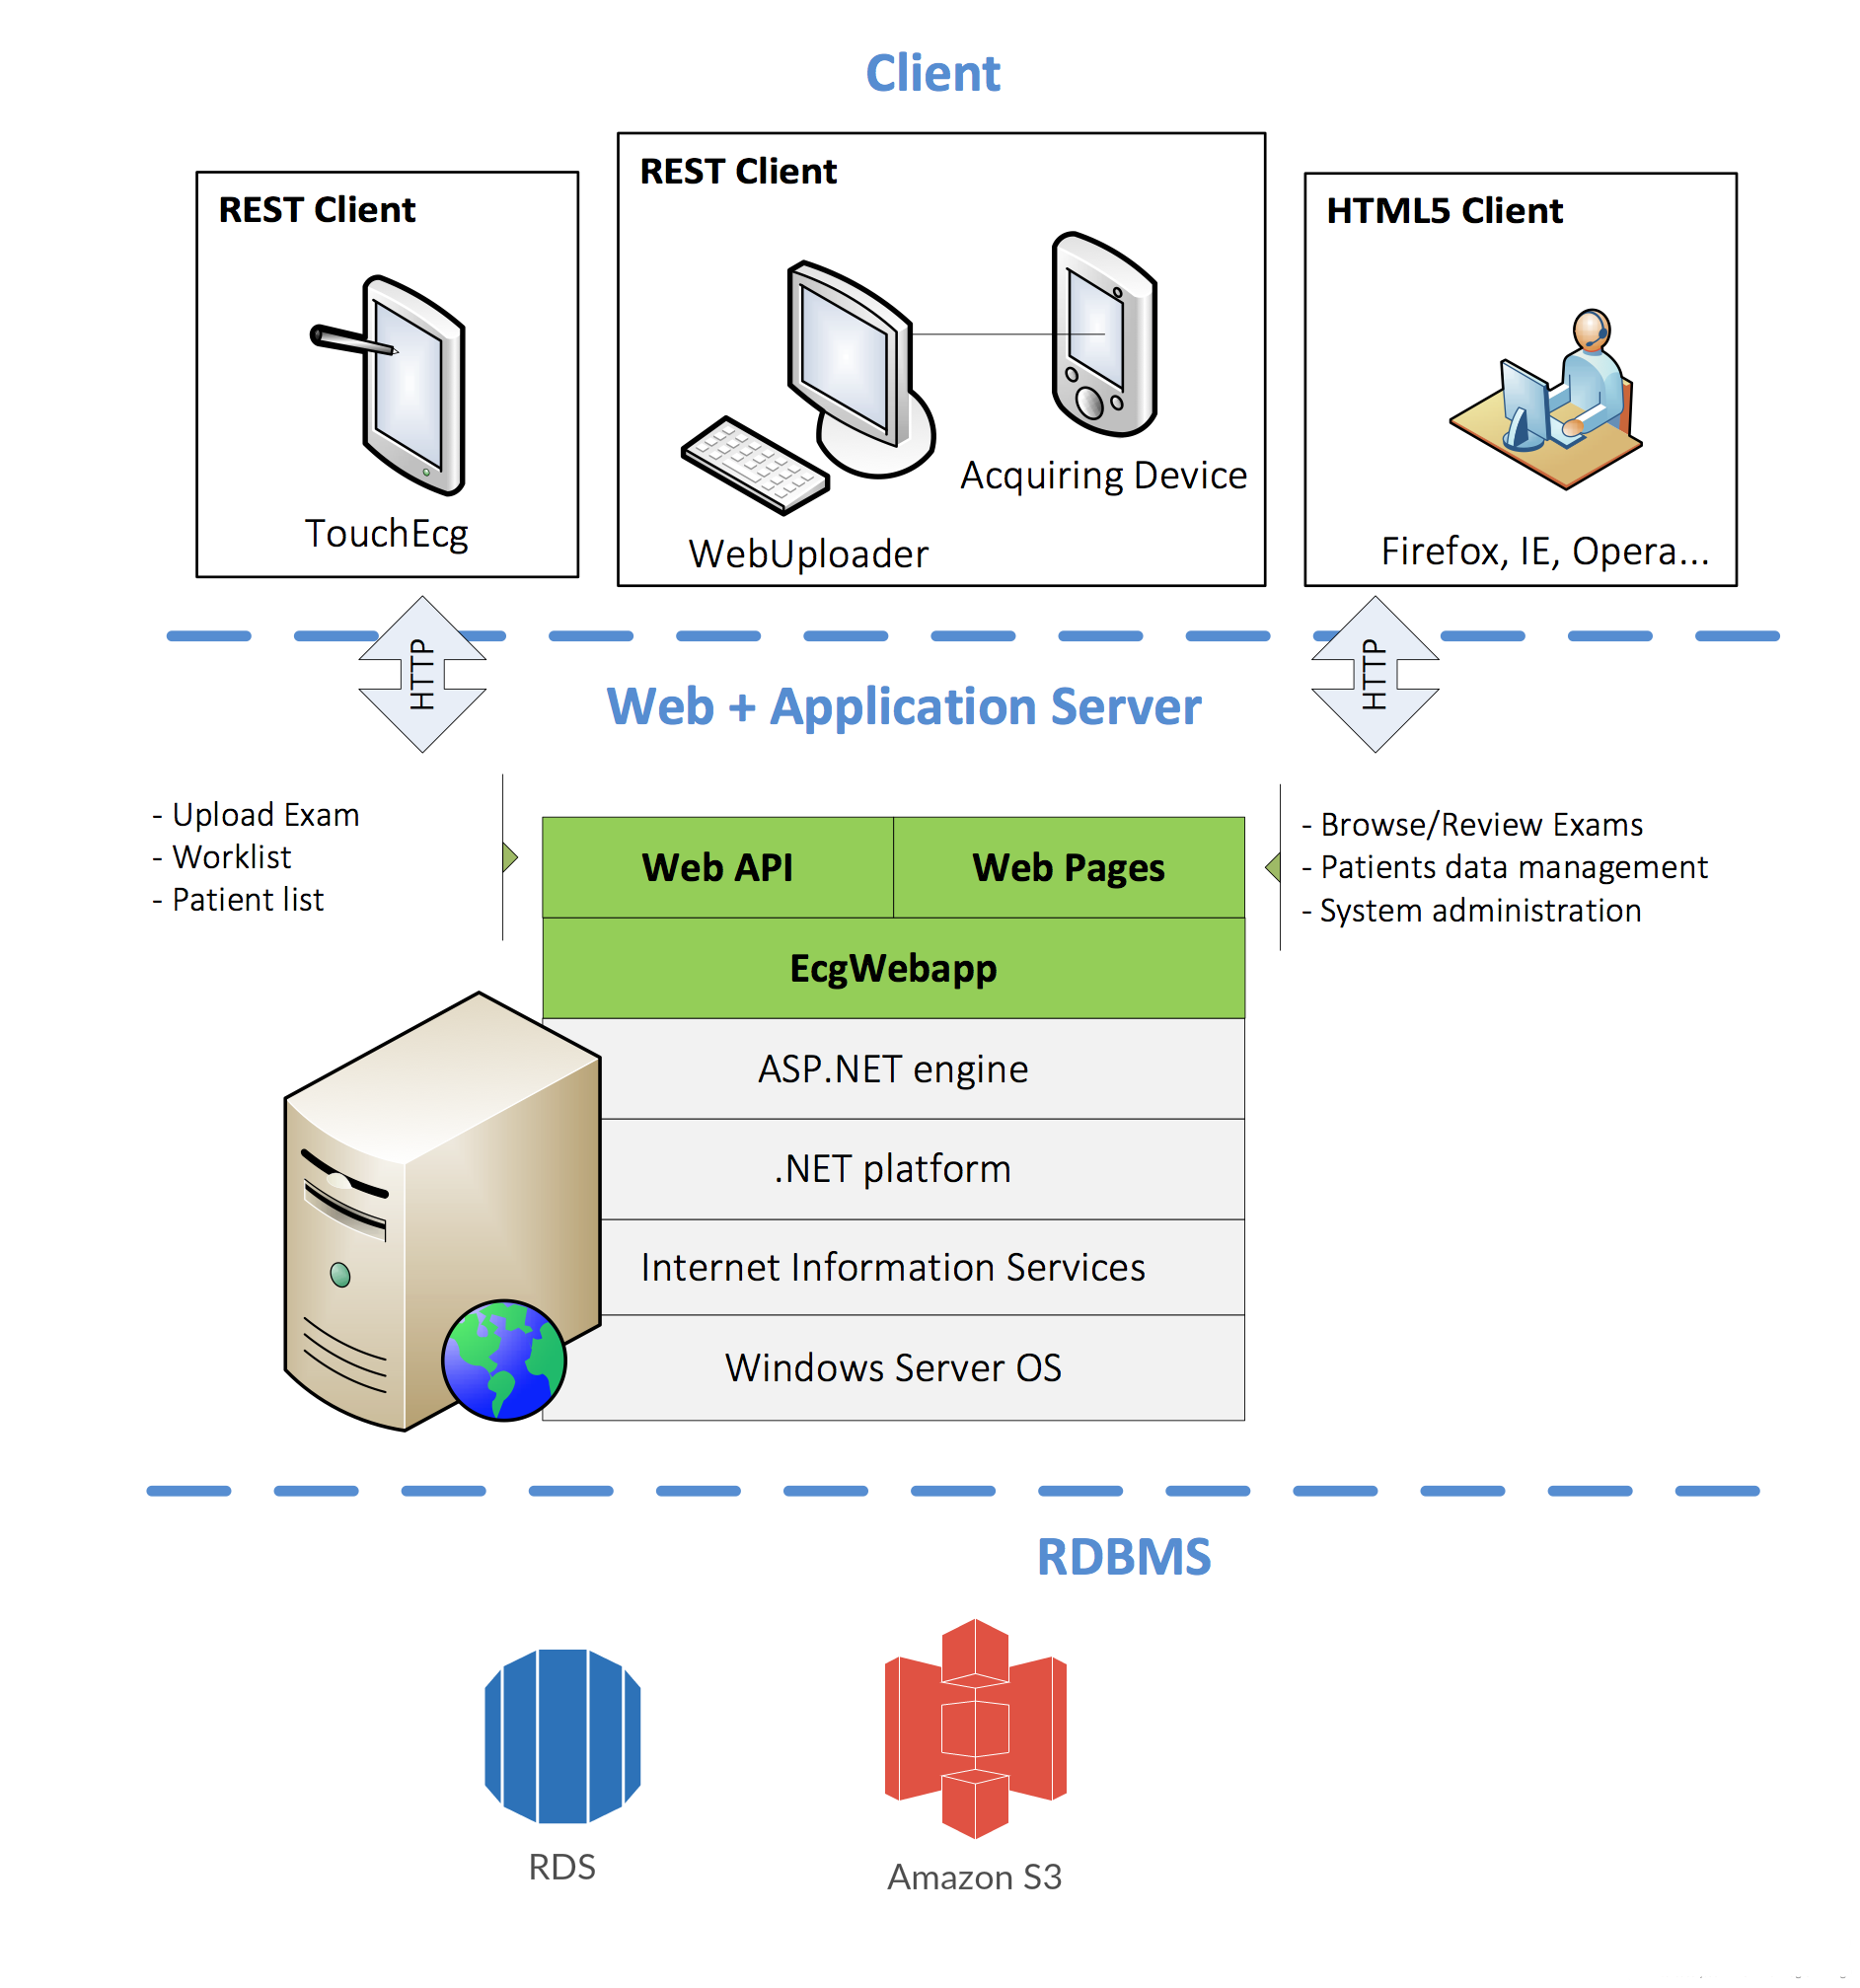
\includegraphics[width=\textwidth,height=10cm,keepaspectratio]{img/tiers_diagram}
    \caption{3-tier architecture}
    \label{fig:tiers_diagram}
\end{figure}
The MVC \textit{(Model View Controller)} paradigm allows to isolate the domain specific logic from the input and presentation ones, making testing and development easier. \cite{mvc}\\
In this specific context the \textit{model} includes objects as exams and patients and their relations, which are mapped to MySql Database Entities by Entity Framework (EF), an open source object-relational-mapping tool (ORM) developed by Microsoft, in order to work without taking care of the underlying database tables and columns where data are actually stored. Indeed developers deal with an higher level of abstraction \cite{wikipedia_ef}.\\
The \textit{view} manages data presentation, serving html pages or json formatted data, as show in figure \ref{fig:app_resource_pattern}.\\
\begin{figure}[h]
    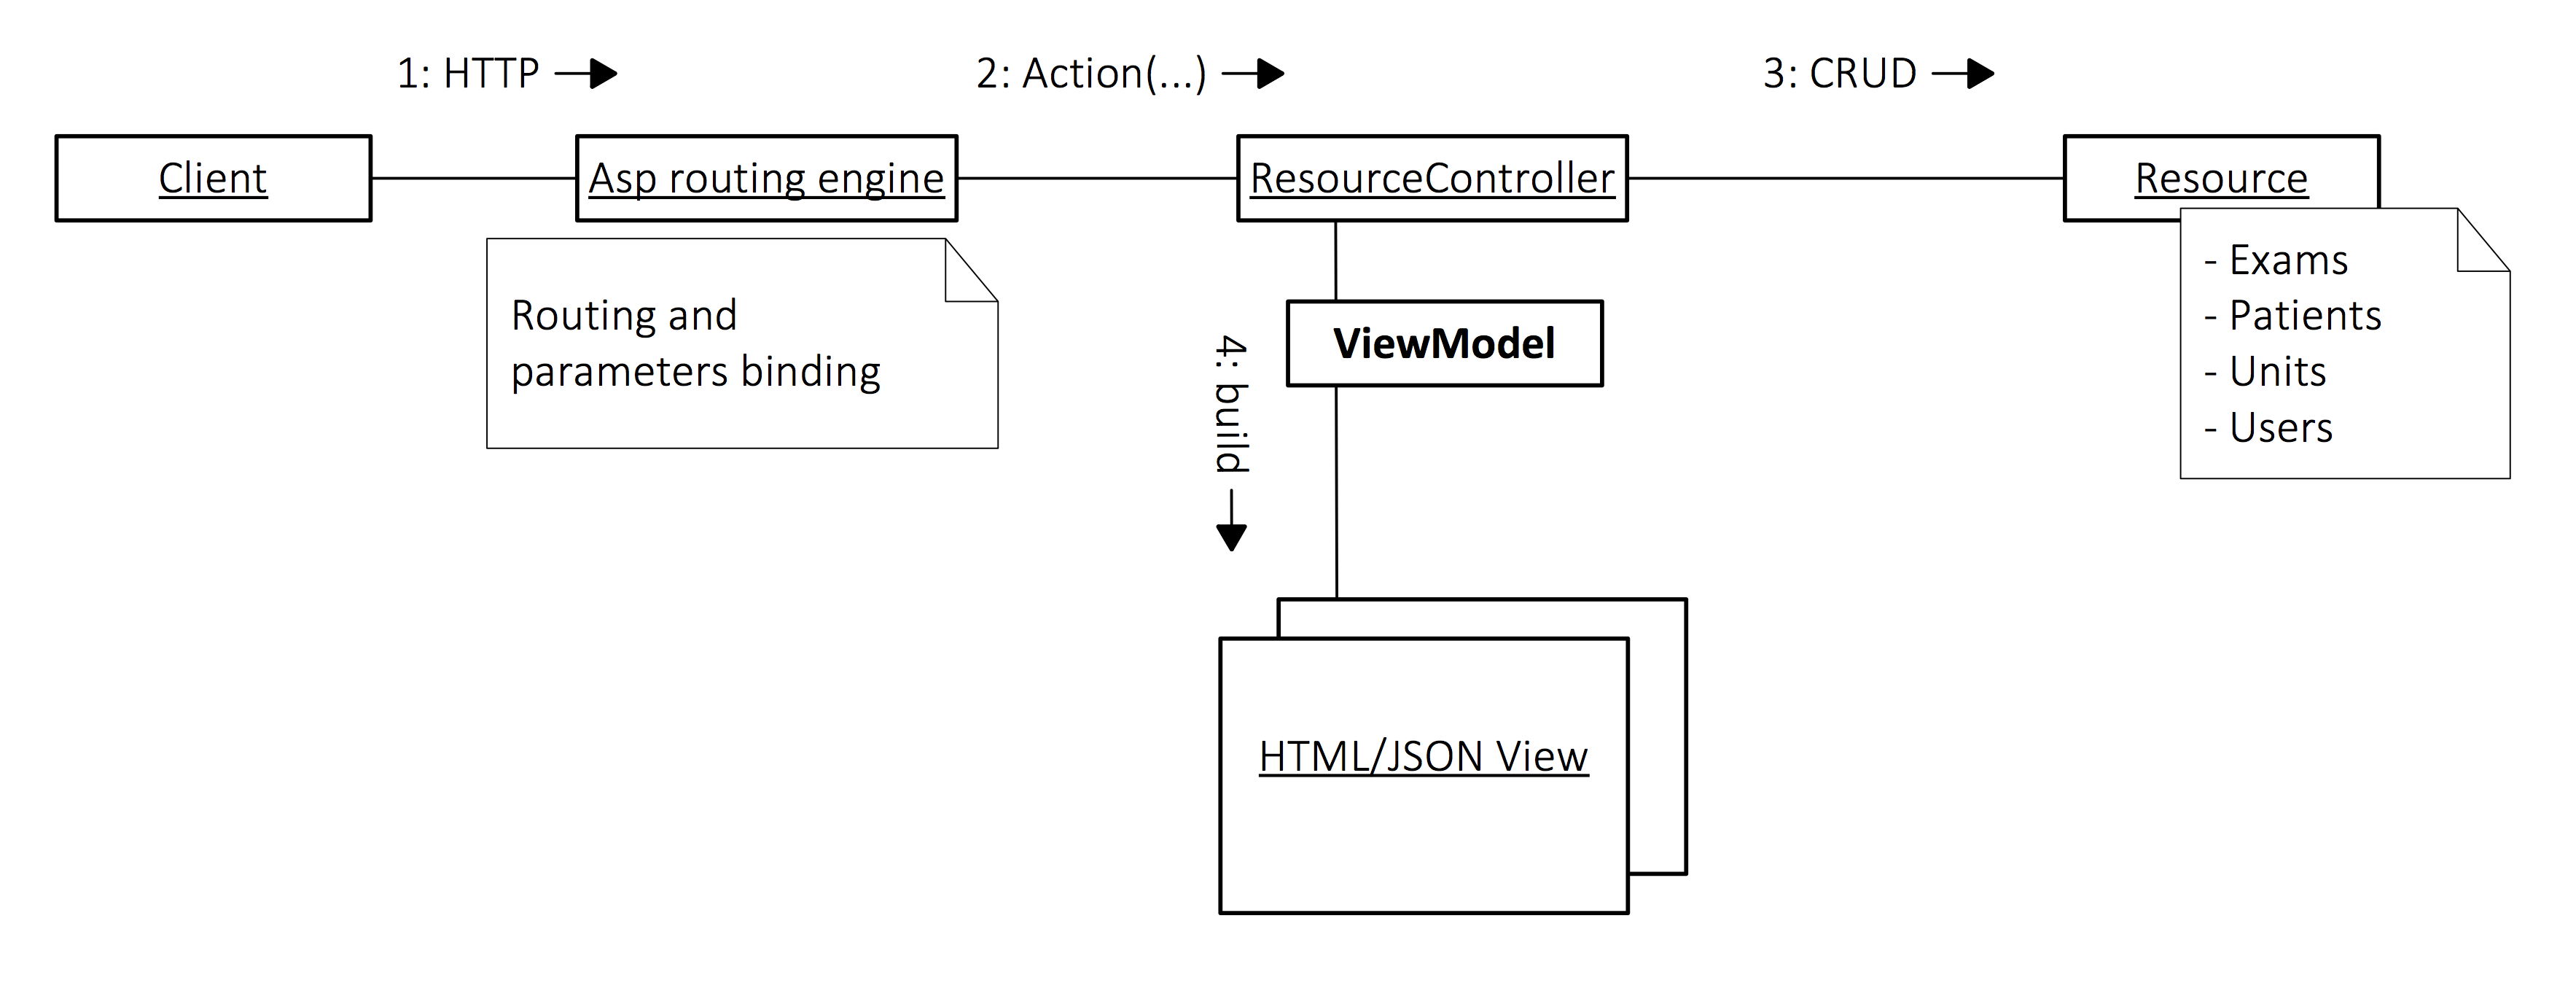
\includegraphics[width=\textwidth]{img/app_resource_pattern}
    \caption{Each application resource has been implemented following this pattern}
    \label{fig:app_resource_pattern}
\end{figure}
WebServices included in EcgWebApp are based on the ASP .NET WebApi Framework: a REST interface triggers a specific action on a resource depending on the URL parameters and the HTTP verb used. Basic Authentication is used to provide access control to web resources.\\ \\
A specific module has been developed to prepare reviewed electrocardiograms for Electronic Health Record. Any time a user with review priviledges confirm his/her analysis, a italian EHR (aka FSE) compliant CDA document (details at \ref{section:interoperability_of_digital_electrocardiograms_data}) is then built and eventually submitted. (EHR - Electronic Healt Record and FSE - Fascicolo Sanitario Elettronico were defined in \ref{subsection:electronic_health_record})
\paragraph{Ecg Web Receiver}
\label{paragraph:ecgwebreceiver}
Similarly to EcgWebApp, (\ref{paragraph:ecgwebapp}) Ecg WebReceiver is an ASP .NET MVC application with a REST webservice module developed with WebApi framework.\\
To receive large files the client must first ask WebReceiver for an upload-session token id, then it starts sending chunks of data until the second last one, each time communicating the uploading session id. Finally the client sends the very last chunk and commits uploading (for a diagram see fig.\ref{fig:holter_sequence_diagram}). Each requests made by client is authenticated server-side from a basic-authentication mechanism. The user is then identified and the exam loaded to the associated bucket on Amazon Simple Storage Service (S3).
The system admin is allowed to login and perform CRUD on users and buckets resources from a web based user interface (screenshot at fig. \ref{fig:webreceiver_admin_screenshot})

\clearpage

\subsection{Clients}
Here is presented a set of client applications which interact with the previously defined components, EcgWebApp (\ref{paragraph:ecgwebapp}) and Ecg WebReceiver (\ref{paragraph:ecgwebreceiver}) over the HTTP protocol.
\paragraph{Touch Ecg}
Touch Ecg is a Cardioline electrocardiograph 12-lead (more details for 12-lead at \ref{subsection:12leadecg}) application for tablet PC: it acquires raw electrocardiograms data from the compatible devices, which are eventually analysed later by the \textit{"Glasgow"} \cite{glasgow} interpretation algorithm.\\
After a configuration phase, where the user is asked to provide the endpoint which the waveforms should be uploaded to, it is possible to transfer ECG-SCP (informations about SCP-ECG file format at \ref{subsection:ecgdigitaliation}) files via a REST WebService (\ref{paragraph:REST}).
\paragraph{Web Uploader}
It is a stand-alone client application developed specifically to save, from Cardioline devices, long time registrations, as Holters are, and upload them. Because of such document's legth an upload protocol has been built to ensure all data will reach the WebReceiver endpoint, illustrated in fig. \ref{fig:holter_sequence_diagram}.
\begin{figure}[h]
    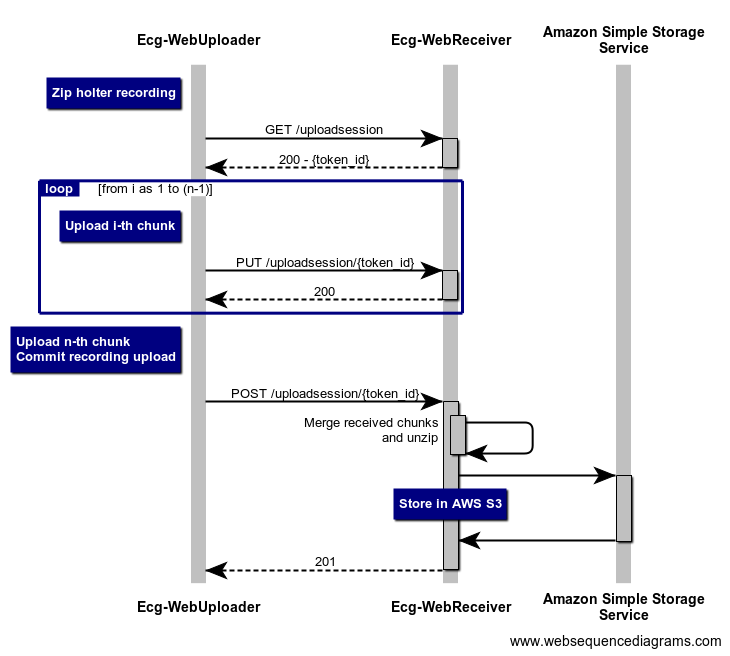
\includegraphics[width=\textwidth]{img/holter_sequence_diagram}
    \caption{Sequence diagram for Holter exams uploading}
    \label{fig:holter_sequence_diagram}
\end{figure}
\paragraph{Browser}
Any browser application can access web pages provided by EcgWebApp (\ref{paragraph:ecgwebapp}). In this way each tenant user is able to login via his/her own computer without installing any additional software, from anywhere.
Here the Ecg-Workflow described in \ref{section:ecgworkflow} is implemented and available to different users.\\
\paragraph{Cube Holter}
An ad hoc software for in-depth holter exam review: given a folder it looks up for the available exams inside.
Because Cardioline tools used to be hosted on a LAN it was easier to deliver directly a long-time heart activity recording to the machine which would be used for the analysis. Given the architectural change carried out, legacy software as CubeHolter have been provided with a module which creates a virtual storage device synchronized with the related Amazon Simple Storage S3 bucket, where exams are exported by WebReceiver (\ref{paragraph:ecgwebreceiver}). Hence the tool is configured to look for exams in such virtual device: the result is a user transparent synchronization mechanism between local machines and cloud even for large files.

\section{Screenshots}

\begin{figure}[h]
    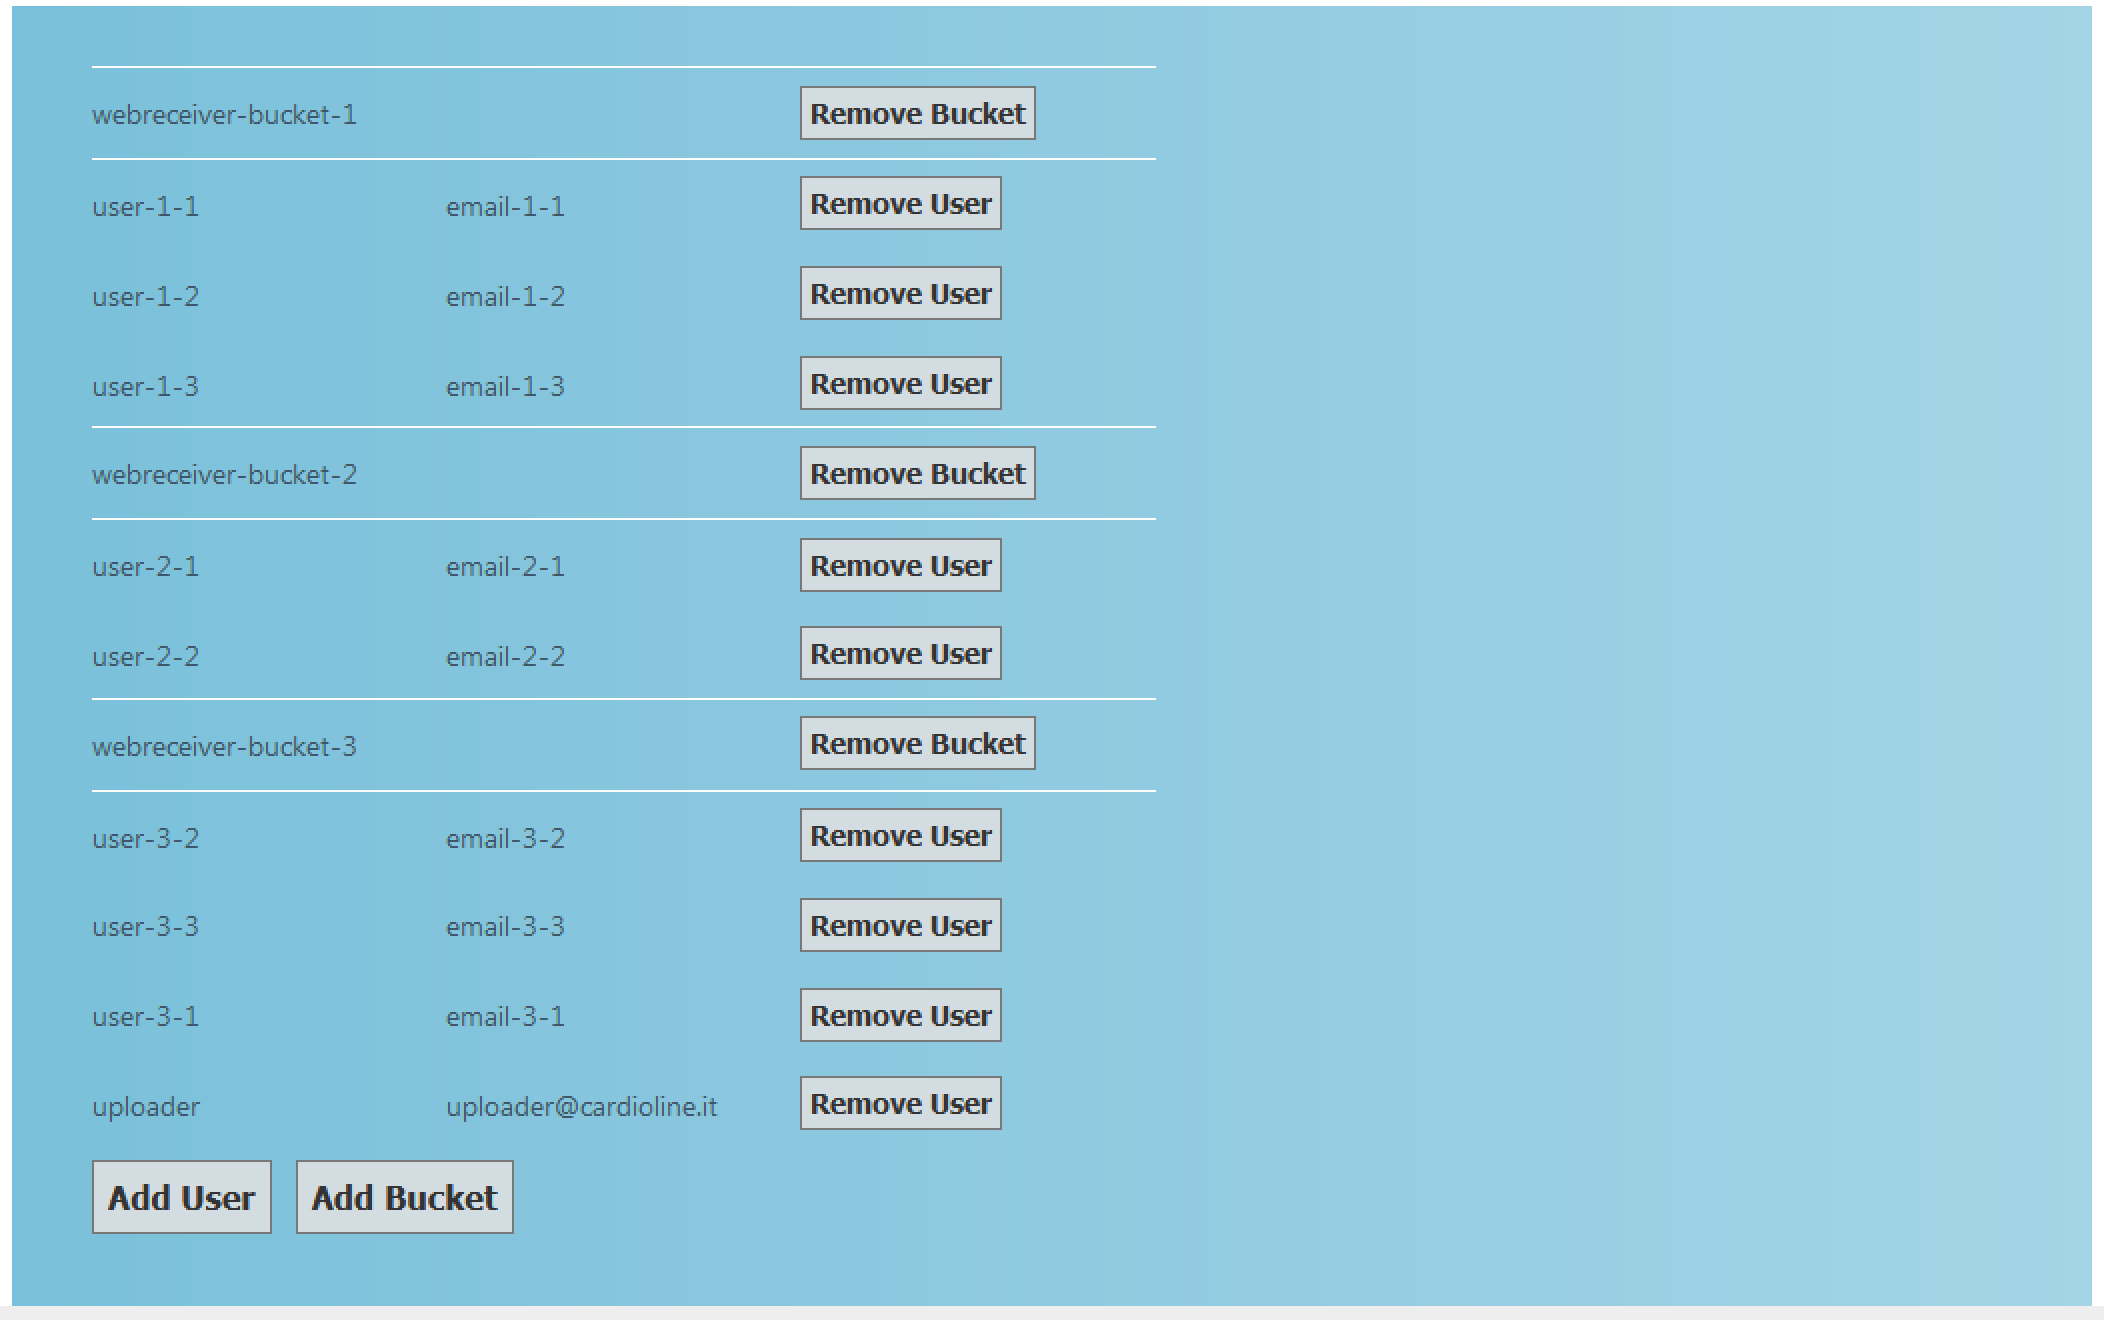
\includegraphics[width=\textwidth]{img/webreceiver_admin_screenshot}
    \caption{Admin user interface for buckets and users management}
    \label{fig:webreceiver_admin_screenshot}
\end{figure}

\begin{figure}[h]
    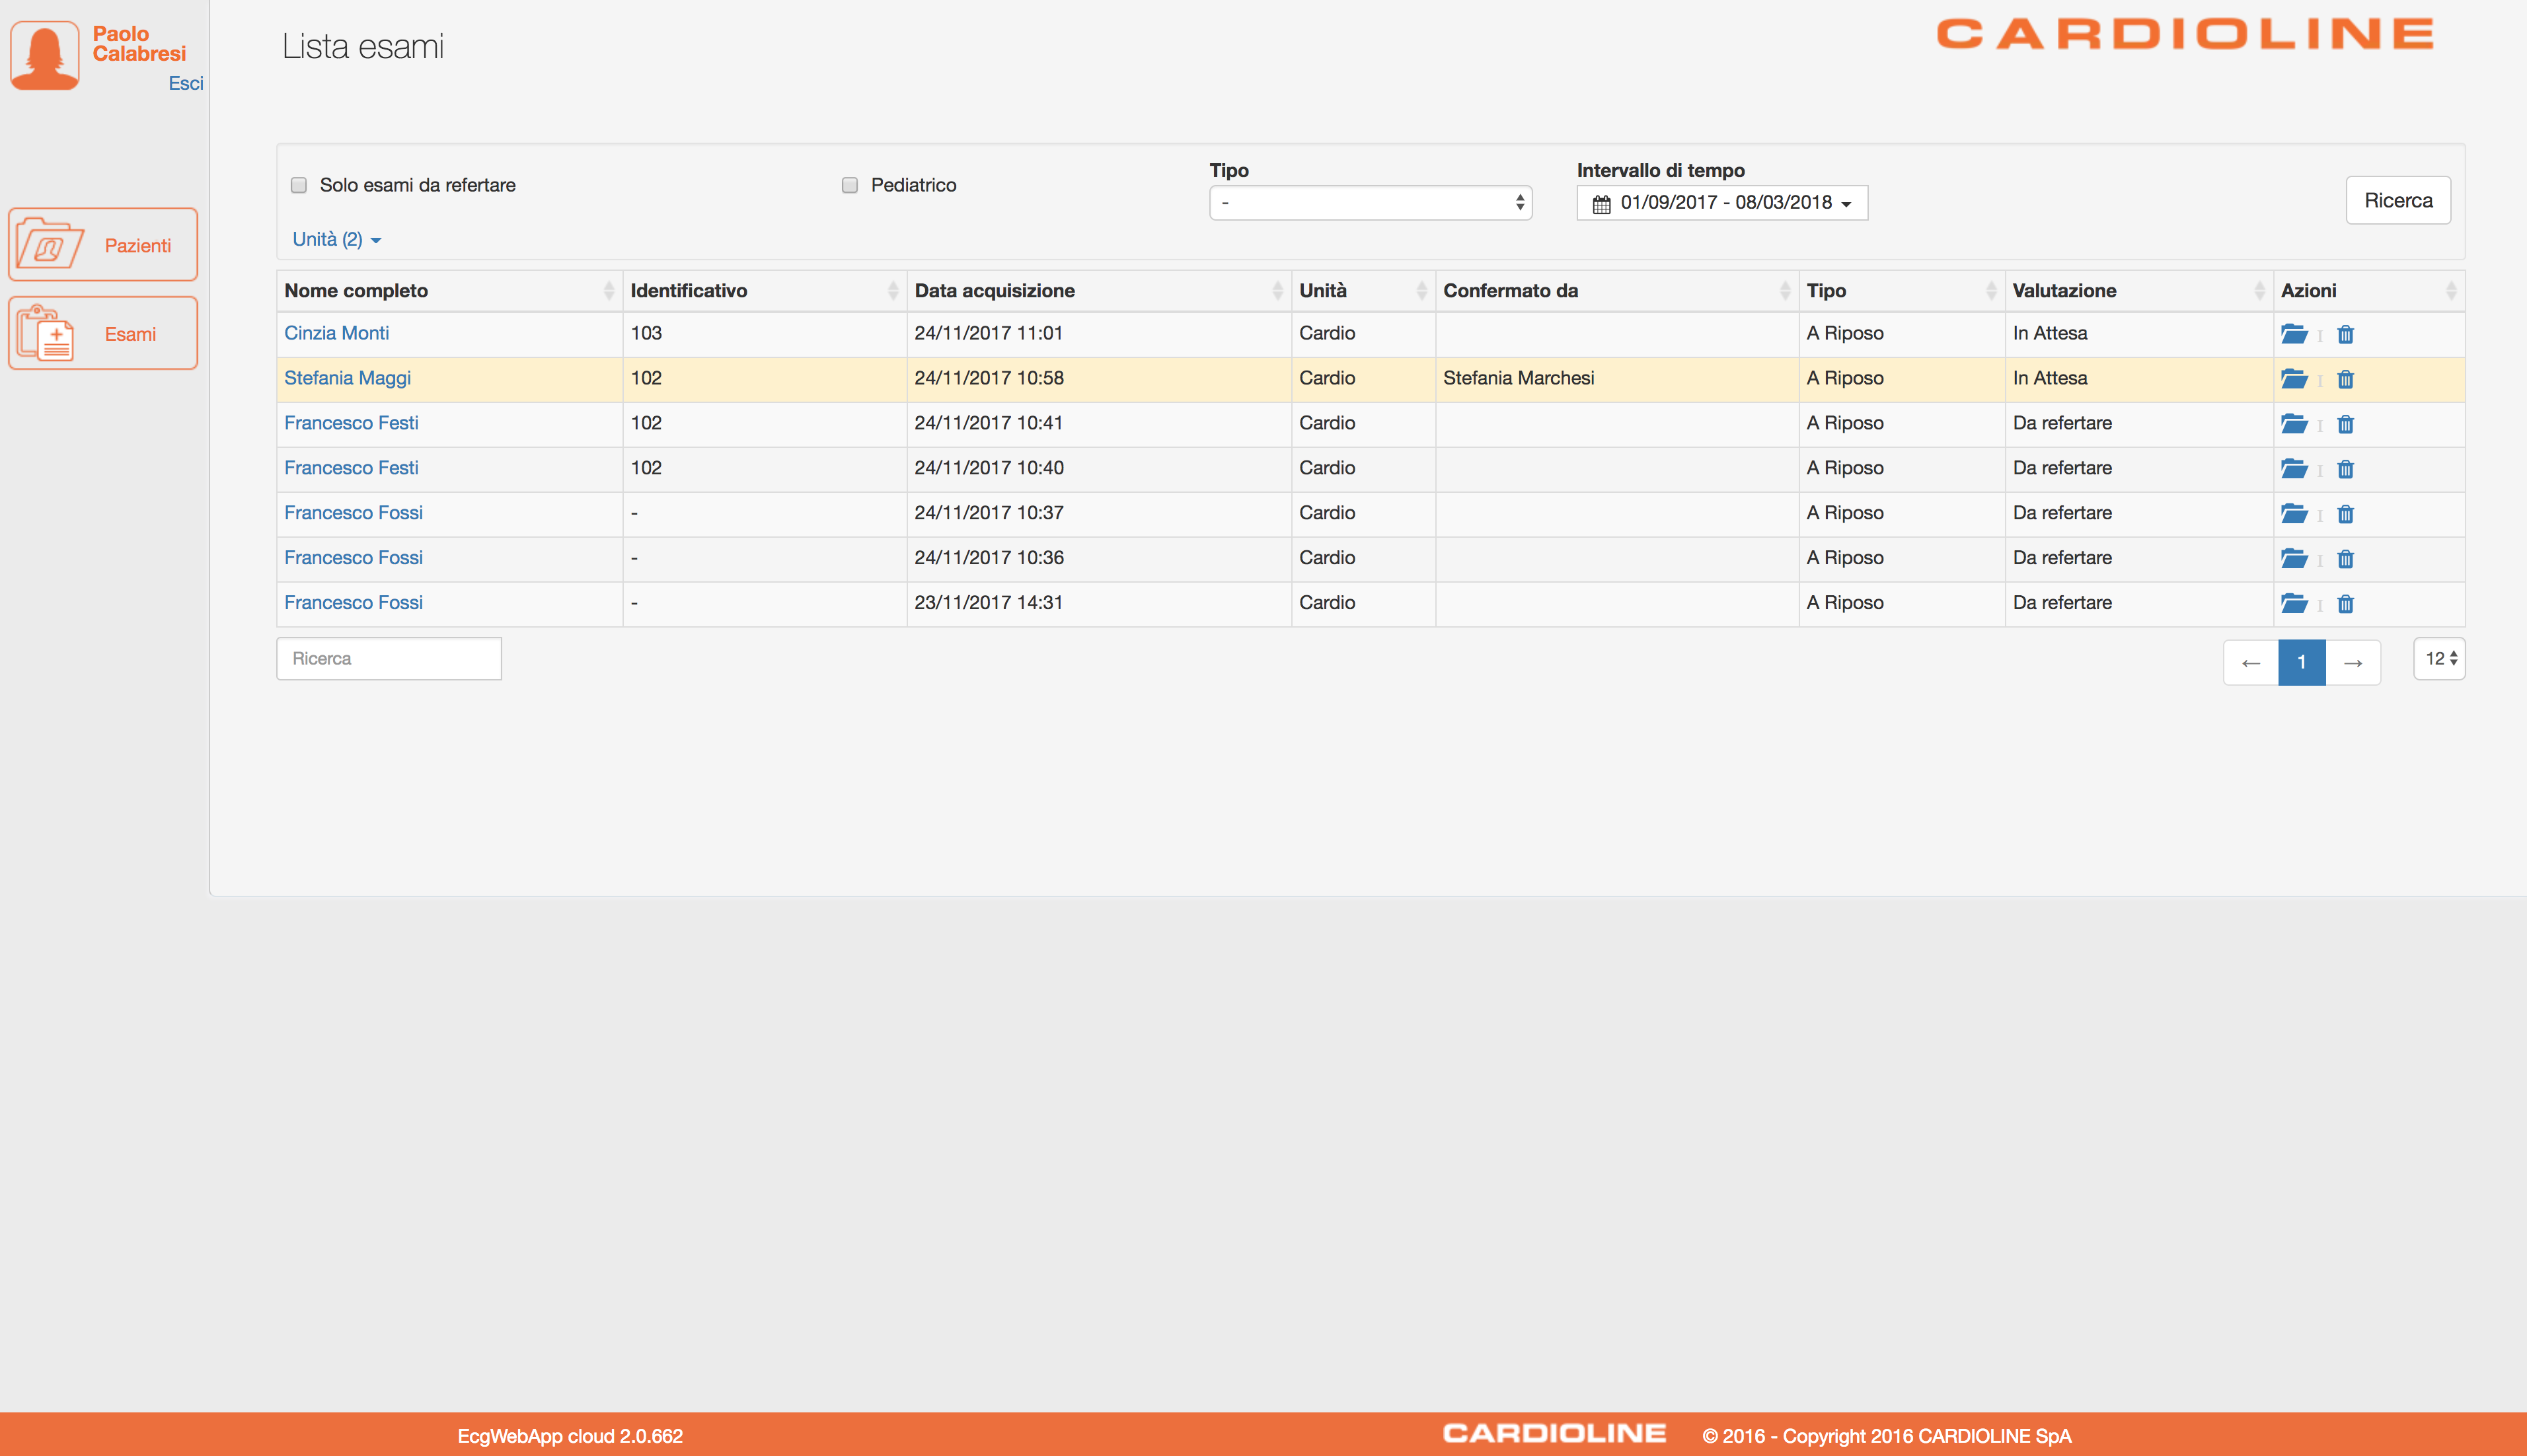
\includegraphics[width=\textwidth]{img/todo_anamnesi}
    \caption{User interface showing anamnesis needed}
    \label{fig:todo_anamnesi}
\end{figure}

\begin{figure}[h]
    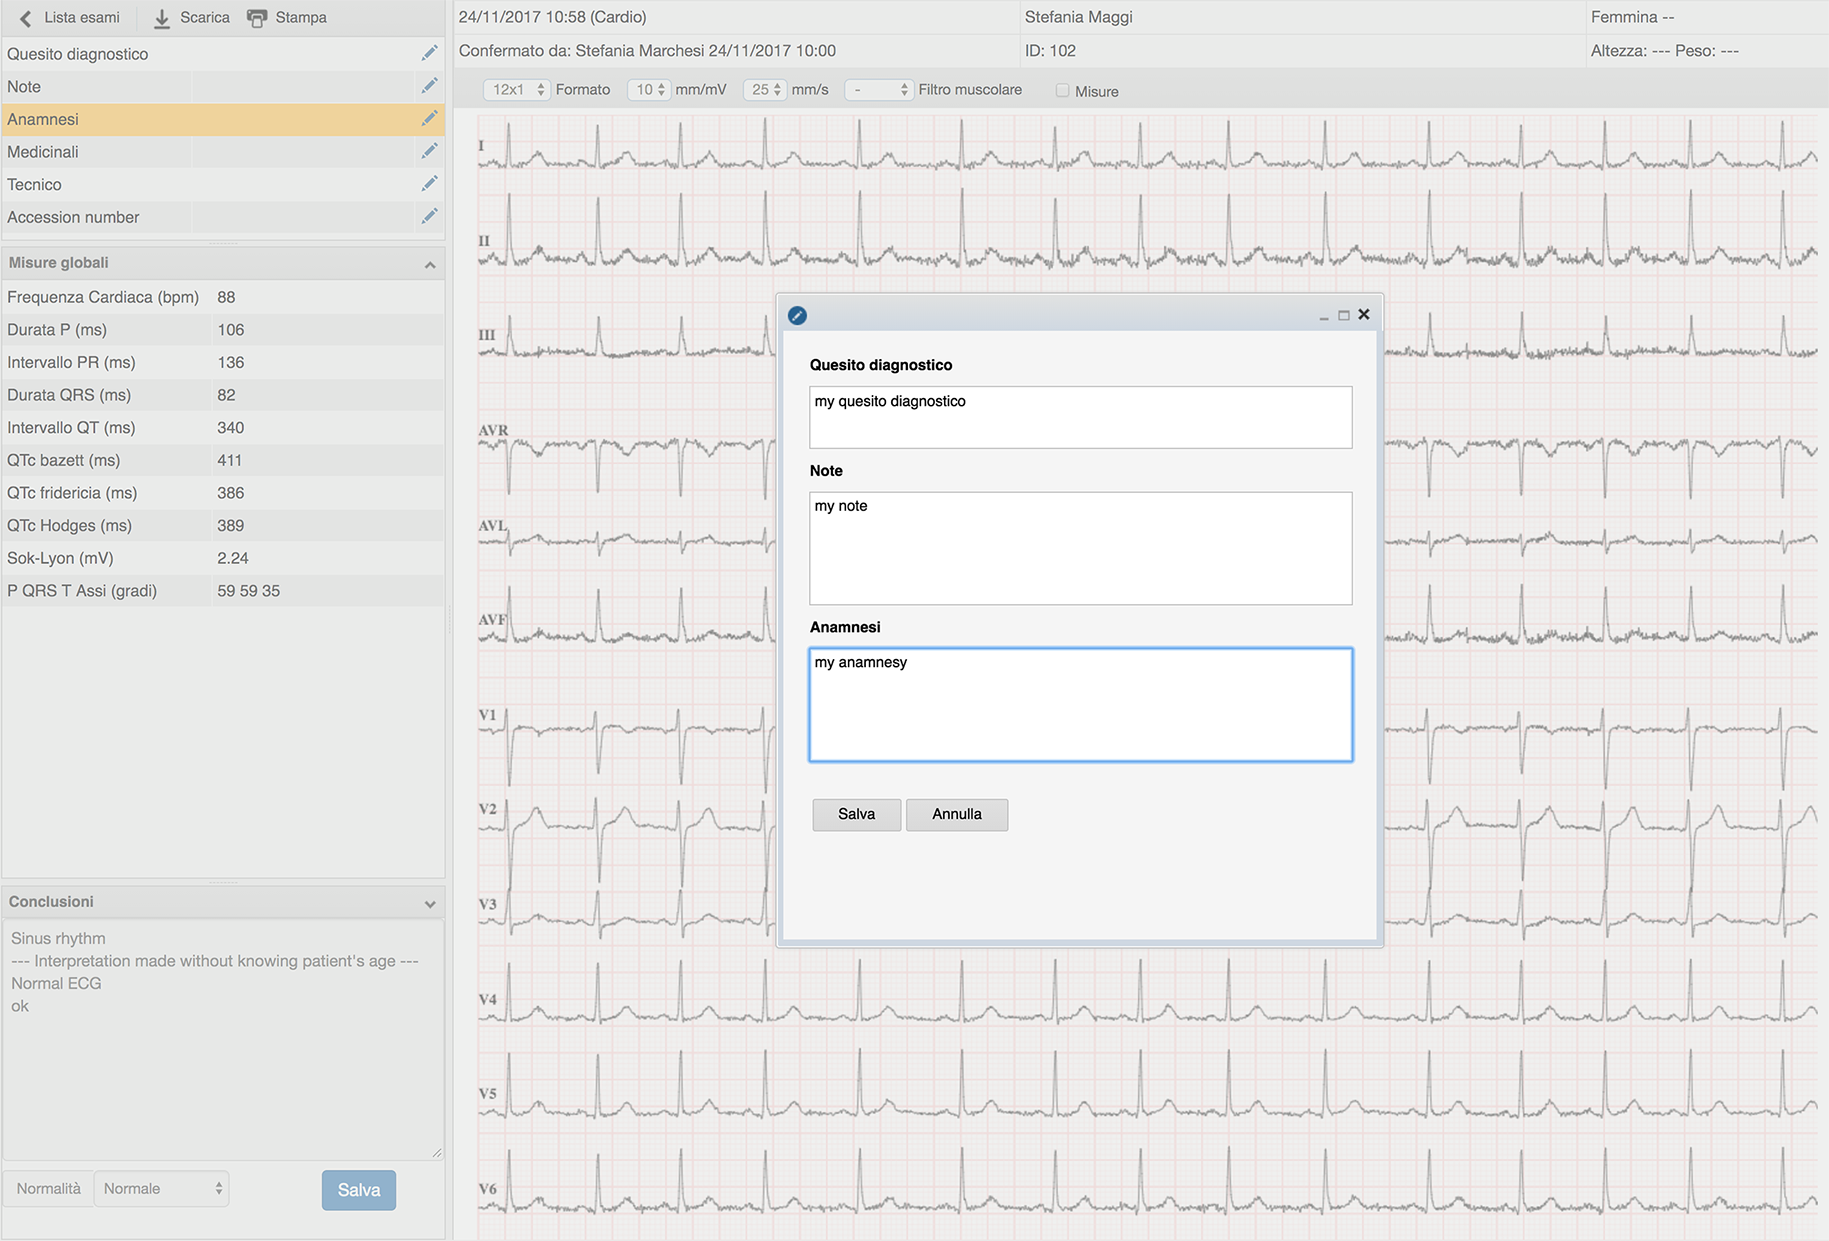
\includegraphics[width=\textwidth]{img/aggiunta_anamnesi}
    \caption{User interface showing anamnesis provisioning}
    \label{fig:aggiunta_anamnesi}
\end{figure}

\begin{figure}[h]
    \includegraphics[width=\textwidth]{img/refertazione_esame}
    \caption{Conclusion provisioning user interface}
    \label{fig:refertazione_esame}
\end{figure}



